\begin{enumerate}
	\item Exercício
	
	Use integral tripla para encontrar o volume do sólido no primeiro octante limitado pelos planos coordenados e pelo plano dado pela equação abaixo.
	
	\begin{equation*}
		3x + 6y + 4z = 12
	\end{equation*}
	
	\begin{figure}[htb]
		\caption{Integrais triplas - Aula 03 - Exercício I}
		\label{v16_a03_e01}
		\centering
		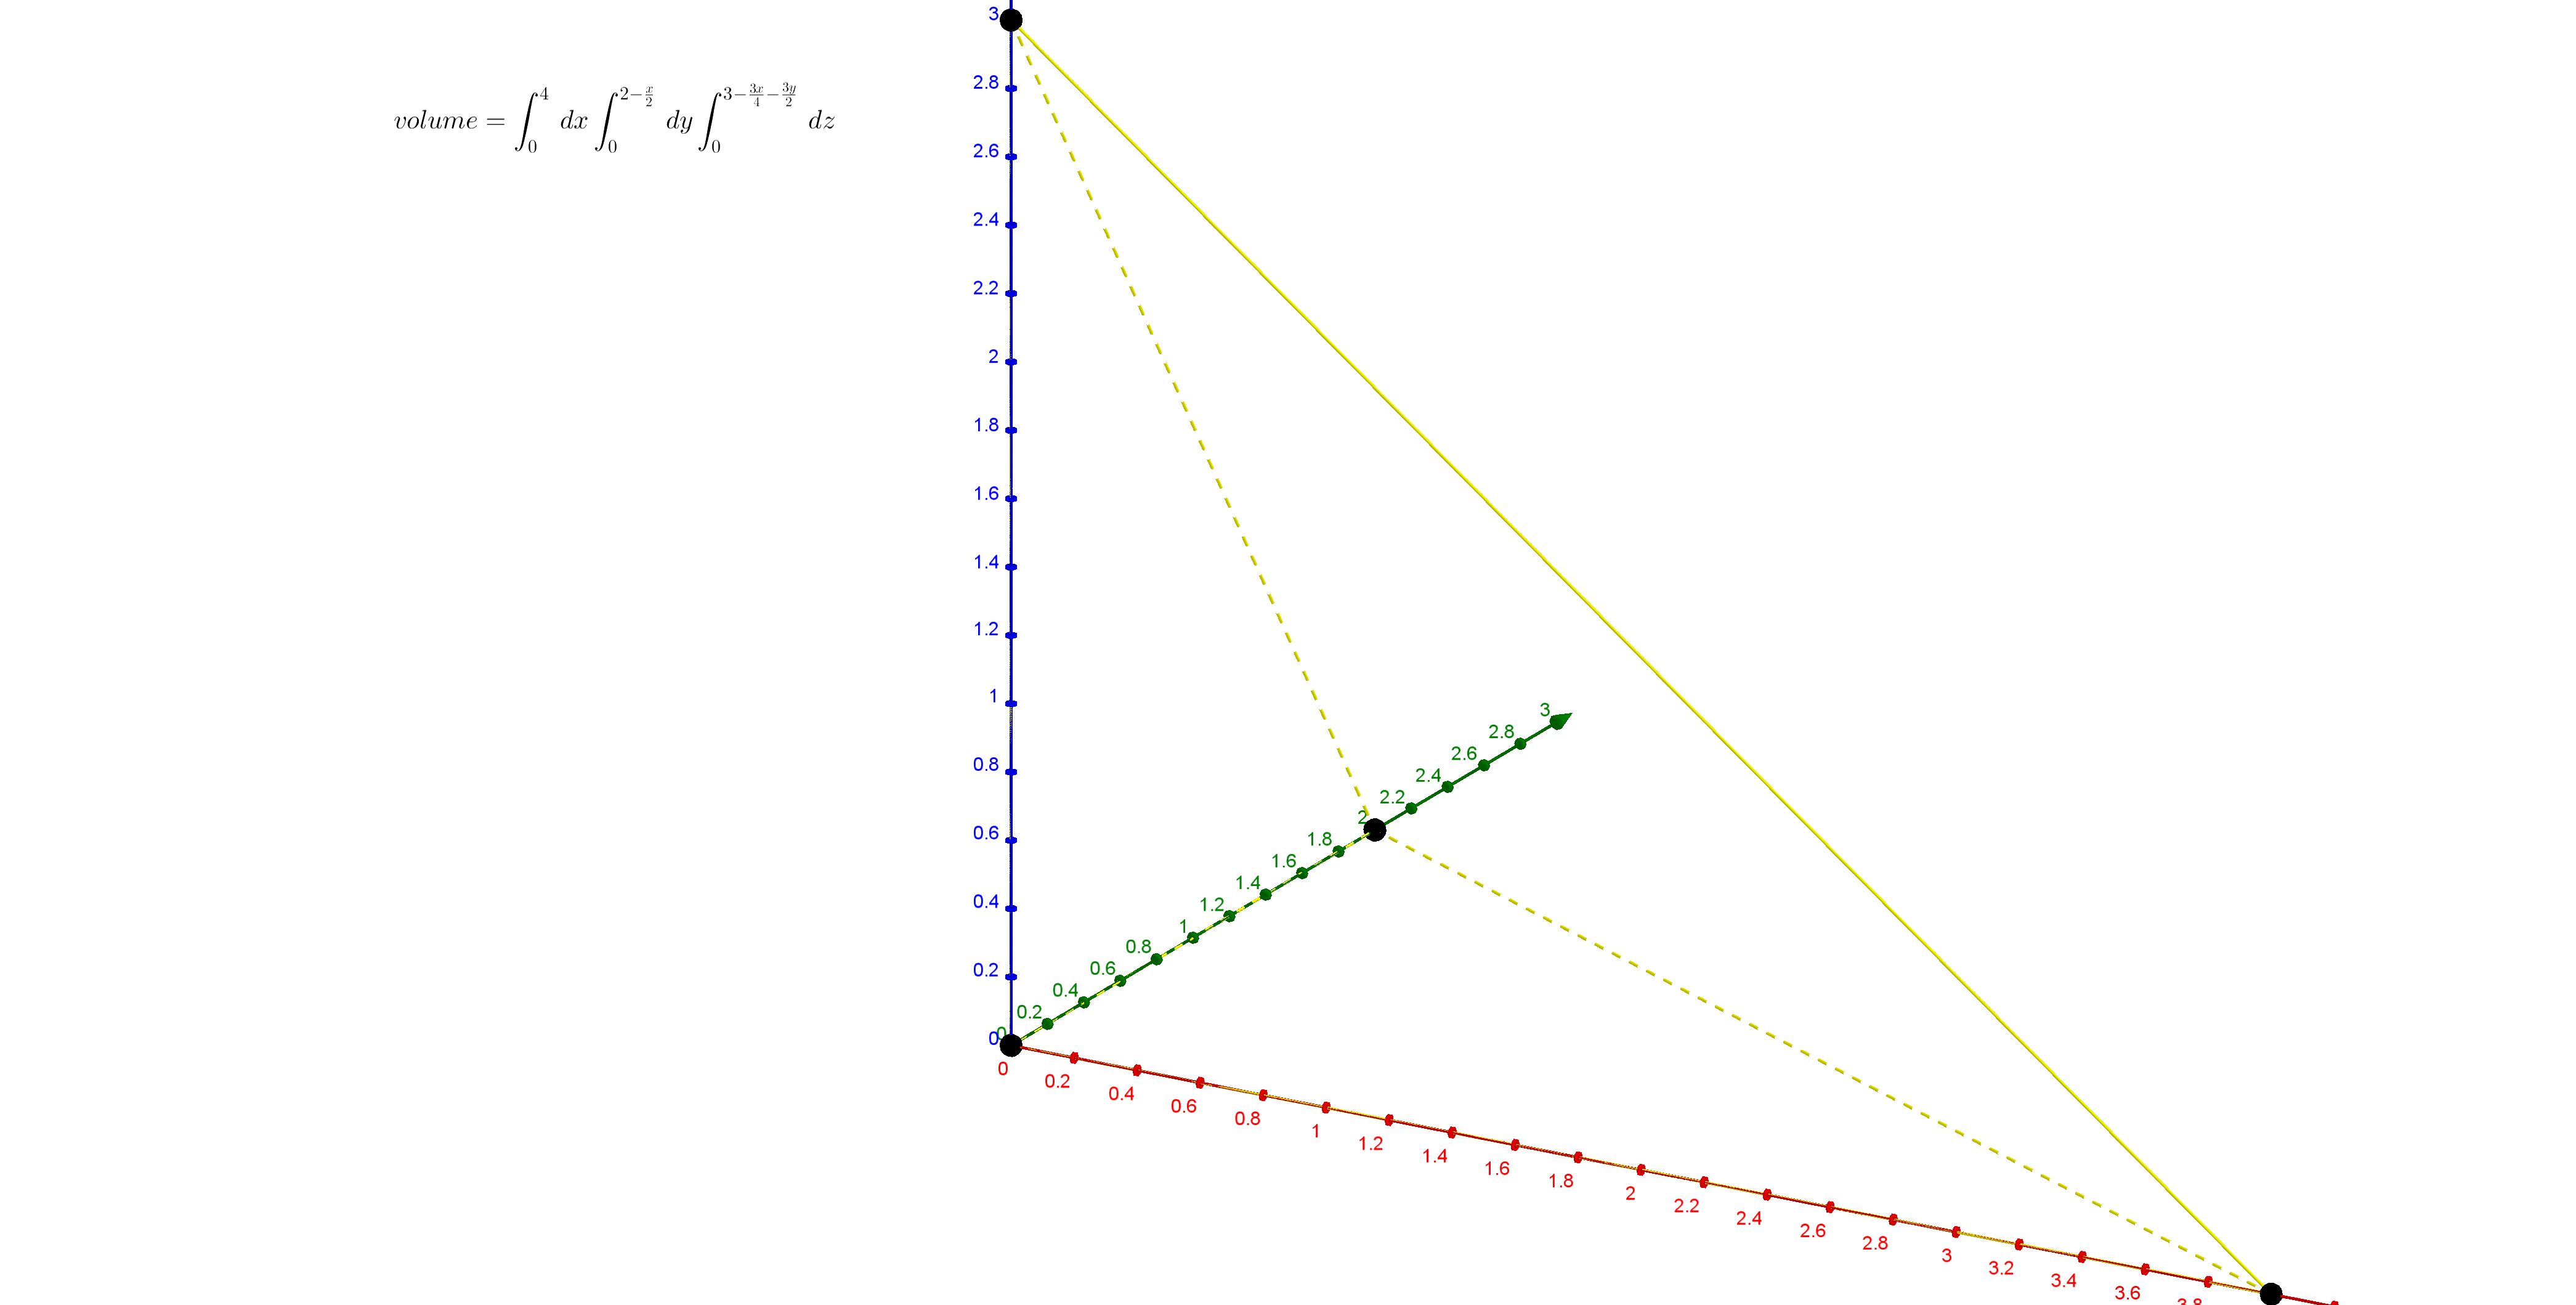
\includegraphics[width=0.5\textwidth]{v16_a03_e01.png}		
	\end{figure}
	
	\begin{equation*}
		P_0(0,0,0) 
	\end{equation*}
	\begin{equation*}
		x = 0,\, y = 0;\; 4z = 12 \Rightarrow z = \dfrac{12}{4}	= 3;\; P_1(0,0,3)
	\end{equation*}
	\begin{equation*}
		x = 0,\, z = 0;\; 6y = 12 \Rightarrow y = \dfrac{12}{6} = 2;\; P_2(0,2,0)
	\end{equation*}
	\begin{equation*}
		y = 0,\, z = 0;\; 3x = 12 \Rightarrow x = \dfrac{12}{3} = 4;\; P_3(4,0,0)
	\end{equation*}	
	
	\begin{equation*}
		0 \leq x \leq 4
	\end{equation*}
	\begin{equation*}
		3x + 6y = 12 \Rightarrow x + 2y = 4 \Rightarrow y = \dfrac{4 - x}{2} = 2 - \dfrac{x}{2};\; 0 \leq y \leq \left(2 - \dfrac{x}{2}\right)
	\end{equation*}
	\begin{equation*}
		3x + 6y + 4z = 12 \Rightarrow z = \dfrac{12 - 3x - 6y}{4} = 3 - \dfrac{3x}{4} - \dfrac{3y}{2} ;\; 0 \leq z \leq \left(3 - \dfrac{3x}{4} - \dfrac{3y}{2}\right)
	\end{equation*}
			
	\begin{gather*}
		 \int_0^4 dx \int_0^{2 - \frac{x}{2}} dy \int_0^{3 - \frac{3x}{4} - \frac{3y}{2}} dz = \int_0^4 dx \int_0^{2 - \frac{x}{2}} dy \left[z\right]_0^{3 - \frac{3x}{4} - \frac{3y}{2}} =\\ \int_0^4 dx \int_0^{2 - \frac{x}{2}} \left(3 - \frac{3x}{4} - \frac{3y}{2}\right) dy = \int_0^4 dx \left[3y - \frac{3xy}{4} - \frac{3y^2}{4}\right]_0^{2 - \frac{x}{2}} =\\ \int_0^4 \left(3\left(2 - \dfrac{x}{2}\right) - \frac{3x\left(2 - \dfrac{x}{2}\right)}{4} - \frac{3\left(2 - \dfrac{x}{2}\right)^2}{4}\right) dx =\\ \int_0^4 \left(6 - \dfrac{3x}{2} - \dfrac{\left(6x - \dfrac{3x^2}{2}\right)}{4} - \dfrac{3\left(4 - 2x + \dfrac{x^2}{4}\right)}{4}\right) dx =\\ \int_0^4 \left(6 - \dfrac{3x}{2} - \dfrac{\left(\dfrac{12x - 3x^2}{2}\right)}{4} - \dfrac{\left(12 - 6x + \dfrac{3x^2}{4}\right)}{4}\right) dx =\\ \int_0^4 \left(6 - \dfrac{3x}{2} - \left(\dfrac{12x - 3x^2}{8}\right) - \dfrac{\left(\dfrac{48 - 24x + 3x^2}{4}\right)}{4}\right) dx =\\ \int_0^4 \left(6 - \dfrac{3x}{2} - \left(\dfrac{3x}{2} - \dfrac{3x^2}{8}\right) - \left(\dfrac{48 - 24x + 3x^2}{16}\right)\right) dx =\\ \int_0^4 \left(6 - \dfrac{3x}{2} - \dfrac{3x}{2} + \dfrac{3x^2}{8} - \left(3 - \dfrac{3x}{2} + \dfrac{3x^2}{16}\right)\right) dx =\\ \int_0^4 \left(6 - \dfrac{\overstrike{3x}}{\overstrike{2}} - \dfrac{3x}{2} + \dfrac{3x^2}{8} - 3 + \dfrac{\overstrike{3x}}{\overstrike{2}} - \dfrac{3x^2}{16}\right) dx = \int_0^4 \left(3 - \dfrac{3x}{2} + \dfrac{3x^2}{16}\right) dx =\\ \left[3x - \dfrac{3x^2}{4} + \dfrac{3x^3}{48}\right]_0^4 = 3\cdot4 - \dfrac{3\cdot4^2}{4} + \dfrac{3\cdot4^3}{48} = \overstrike{12 - 12} + 4 = 4
	\end{gather*}	
\end{enumerate}